\def\year{2017}\relax
%File: formatting-instruction.tex
\documentclass[letterpaper] {article} %DO NOT CHANGE THIS
\usepackage{aaai17}  %Required
\usepackage{times}  %Required
\usepackage{helvet}  %Required
\usepackage{multirow}
\usepackage{courier}  %Required
\usepackage{url}  %Required
\usepackage{graphicx}  %Required
\usepackage{tcolorbox}

\usepackage{csquotes} %Added from CSCW Paper
\usepackage{comment}
\frenchspacing  %Required
\setlength{\pdfpagewidth}{8.5in}  %Required
\setlength{\pdfpageheight}{11in}  %Required
%PDF Info Is Required:
  \pdfinfo{
/Title			
/Author (AAAI Press Staff)}
\setcounter{secnumdepth}{0}  
 \begin{document}
% The file aaai.sty is the style file for AAAI Press 
% proceedings, working notes, and technical reports.
%
\title{AI behind conversational bots}
\author{Nalin Chhibber\\ Student ID: 20715659, MMath CS(HCI)}
\maketitle
\begin{abstract}
The primary aim of this paper is to describe popular techniques that researchers have been using to build voice user interfaces and cover a sizable body of literature related to the area. Additionally, this paper replicates the results by \cite{lowe2015ubuntu} for Unstructured Multi-Turn Dialogue Systems. Based on the findings, the paper also introduces a new conversational agent: nBot. nBot is trained on a limited dataset of manually constructed sentences and build witt combination of both retrieval-based and generative techniques. It uses Long Short Term Memory to remember the context of conversation.
\end{abstract}

\section{Introduction}
%\begin{figure}[ht]
%\centering
 % 
\includegraphics[width=0.8\columnwidth]{figures/sample.jpg}
%\caption{Lorem ipsum dolor sit amet, consectetur adipiscing elit, sed do eiusmod tempor incididunt ut labore et dolore magna aliqua. Ut enim ad minim \textit{veniam}, quis nostrud exercitation ullamco laboris }
%\label{fig:workflow}
%\end{figure}
As we are gradually incorporating technology in our lives, we are also trying to simplify the interaction technique by getting rid of unused mediums from the space of complicated interfaces. Taking the example of a simple phone, we started using them with rotary dials, then replaced those with numeric buttons and moved on to using touch screens. Voice user interaction is the next logical step and we have already started seeing a glimpse of it in Siri and Google Assistant. While most of the existing modes of human-computer interaction (touch/type/click) require users to adapt with the interface(screen/keyboard/mouse), voice user interfaces on the other hand, comes natural to humans and hence can be used as one of the most promising medium to engage them in a productive interaction. There has been a lot of optimism in the thought that near future will witness a rapid growth in human-computer-interaction using voice. This has not only led to an increased demand of conversational agents but also shown an increase in various chatbot development frameworks. Brands are increasingly using chatbots to engage their customers. Within just a couple years, we have seen a different evolution in the design of conversational agents from chatbots in Facebook Messenger, to Siri in iphones, to Microsoft's Cortana, Google Home and Amazon Alexa. While we cannot predict when Watson or Siri will start working like Jarvis, there is a still a lot that we can do with the normal scripted conversational agents.\\\\
This paper has implemented a simple conversational agent, nBot using a combination of retrieval-based and generative models. It uses a recurrent neural network with 4 hidden layers of LSTM cells to understand the context and respond to user utterances. It has been trained on a limited dataset of manually constructed conversations over 5000 epochs.\\\\
Rest of the paper describes taxonomy of models, major challenges and related work around the design of conversational bots.  It then details the implementation of nBot, followed by discussions on future work.

\section{Taxonomy of models}
%The term 'chatbot' covers a number of categories including stand-alone applications, AI tools, bot developer frameworks, messaging services, bot discovery, and analytics. This paper is mainly concerned with version that defines them as conversational agents.
\subsection{Retrieval based vs Generative vs Pattern based}
Challenge of building a conversational bot can be addressed using a retrival-based, generative or pattern-based model. Retrieval-based models are those which have a repository of pre-defined responses to answer a user utterance. Alicebot and Cleverbot are examples of such types. On the other hand, generative models are those which can generate responses they have never seen before. Microsoft's Tay bot is an example of generative model. Generative models are usually based on machine translation techniques but instead of translating from one language to another, they translate from input uttrance to output response. Both approaches have some obvious pros and cons. Retrieval based techniques dont make gramatical mistakes and are easier to train due to repository of handcrafted rules. However they may be unable to handle unseen cases for which no appropriate response exists. For the same reason these models cant refer back to contextual entity information. Generative models overcome this limitation and can refer back to entities in the input. However these models are harder to train, likely to make gramatical mistakes, produce inconsitant or irrelevant responses and require huge amounts of training data.  %For these reasons most of the production system these days are either retrieval based or a combination of both.
\\\\
Another technique is to use pattern-based heuristics for selecting a response. In these techniques, when the agent receives a message, it goes through all the patterns until it finds a pattern which matches user utterance. If the match is found, the chatbot uses the corresponding template to generate a response. The problem with pattern-based heuristics is that patterns should be programmed manually which is not easy, especially if the agent has to correctly distinguish hundreds of intents. Users can express the same intent in many ways or use similar words in different contexts. Machine learning can help us train an intent classificaltion algorithm to pick patterns in the data. Most of the existing chatbot frameworks(wit.ai, dialogflow, Microsoft LUIS) are based on this technique.

\subsection{Open-domain vs Close-domain}
In open-domain, conversations dont have a well defined goal or intention and can jump to any topic from dating to space travel to politics. Conversations on social media sites like Reddit and Twitter are typically open domain. In closed domain, space of possible input utterance is limited to a specific topic(education, casual conversation, technical support). It is realtively easy to model a conversational agent in close domain. Figure 1 illustrates relative difficulity in designing chatbots with different techniques.
\begin{figure}[ht]
	\centering
	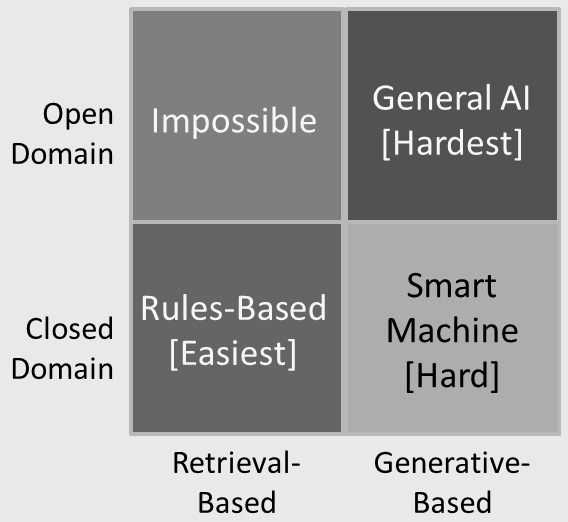
\includegraphics[width=200px]{figures/chatbots.png}
	\caption{Chatbot Conversation Framework\cite{chatbot:framework}}
	\label{fig:chatbotframework}
\end{figure}
\subsection{Online vs Batch Learning}
Batch learning generates the best predictor by learning on the entire training data set at once. Online learning on the other hand uses new responses to update the best predictor for future responses at each step. Online learning can dynamically adapt to new patterns in the conversation as it is generated as a function of time. One problem with online learning is to control unwanted or potentially harmful information. One significant instance is when Microsoft's Twitter chatbot: Tay, started posting a deluge of incredibly racist messages in response to questions. Tay was designed to learn from conversations and get progressively "smarter" but online troublemakes and trolls persuaded it to blithely use racial slurs and even outright call for genocide \cite{microsoft:tay}. Therefore online learning should be assisted by other techniques to prevent them from going off the rails.

\subsection{End-to-end vs Distributed Learning}
Distributed learning systems require multiple stages of processing and follow a set pipeline for solving tasks at hand from feature extraction to learning the desired result. End-to-End learning on the other hand omits any hand-crafted intermediatery algorithms and directly learns the solution to a given problem from sampled dataset. This could involve concatenation of different neural networks(CNNs, RNNs) which are trained simultaneously. The idea is to let the network go from"raw-est" possible data to "final-most" output.
\section{Challenges}
\subsection{Context Awareness}
In real conversations, people don't start thinking from scratch every second to come come up with a new response. They build the conversation based on relevant concepts they might have discussed in past. Therefore, to produce sensible responses systems may need to incorporate both linguistic context and physical context. The most common approach is to embed the conversation into a vector, but doing that with long conversations is challenging in simple recurrent neural networks. Experiments by \cite{serban2016building} and \cite{yao2015attention} both go into that direction. Besides maintaining the context of topic, a smart conversational agent should also incorporate other kinds of contextual data such as date/time, location and information about a user.

\subsection{Consistent Personality}
When generating responses the agent should ideally produce consistent answers to semantically identical inputs. For example, the response to inputs like "How old are you?" and "What is your age?" should be same. This might sound simple, but incorporating such fixed knowledge or "personality" into models is very much a research problem. Since most of the models are trained on data from multiple different users, they tend to give inconsistent responses to the same user utterance. Works like \cite{li2016persona} has proven to be first steps into the direction of explicitly modeling a personality in a conversational bot.
\subsection{Evaluation of Models}
The ideal way to evaluate a conversational agent is to measure whether or not it is fulfilling its task.However such labels are expensive to obtain as there is no well-defined goal. Common metrics such as BLEU(Bilingual Evaluation Understudy) that are based on text matching and used for Machine Translation aren’t well suited because sensible responses can contain completely different words or phrases. In \cite{liu2016not}, authors have concluded that none of the commonly used metrics really correlate with human judgment.
\subsection{Intention and Diversity}
One of the prime issues with most fo the retrieval-based and generative models is lack of diversity in responses. Google's smart reply is a good example of this whose earlier version used to respond with "I love you" to almost anything. This is partly due to how these systems are trained, both in terms of data and in terms of actual training objective/algorithm.  Some researchers have tried to artificially promote diversity through various objective functions \cite{li2015diversity}. Humans conversations are typically specific to the input and carry an intention. Since generative models aren’t trained to have specific intentions they lack this kind of diversity.
\subsection{Choice of corpus}
A corpus is a principled collection of texts, written or spoken, which is stored on a computer. It must represent something and its
merits are often judged based on how representative it is. There are many corpora available and some can be bought, some are free and some are not publicly available. There is no one corpus to suit all purposes and choice of corpora is really important while training a conversational agent for a specific purpose \cite{o2007corpus}. Some popular corpus that have been used to train conversational bots are as follows:
\begin{itemize}
	\item NPS Chat Corpus: Consists of 10,567 posts in release 1.0. It is a part of python NLTK package.
	\item NUS Corpus: Collection of SMS messages compiled by NLP group at National University of Singapore.
	\item Ubuntu Dialogue Corpus: Consists of 1,000,000 examples based on chat logs from the Ubuntu channels on a public IRC network.
	\item Cornell Movie-Dialogs Corpus:  Contains a large metadata-rich collection of fictional conversations extracted from raw movie scripts: 220,579 conversational exchanges between 10,292 pairs of movie characters.
	\item Microsoft Research Social Media Conversation Corpus: Collection of 12,696 Tweet Ids representing 4,232 three-step conversational snippets extracted from Twitter logs.
\end{itemize}
For an effective research in dialog systems, corpus should have following qualities:
\begin{itemize}
	\item Two-way (or dyadic) conversation, as opposed to multi-participant chat.
	\item Large number of conversations.
	\item Many conversations with several turns(more than 3).
	\item Task-specific domain, as opposed to chatbot systems.
\end{itemize}
Most of these requirements are satisfied by the Ubuntu Dialogue Corpus introducted by \cite{lowe2015ubuntu}. Following section describes the related work in the development of conversational agents but focus specifically on \cite{lowe2015ubuntu}, and report replicated results using their technique.
\section{Related work}
Typical dialogue systems consist of a Speech Recognizer, Language Interpreter, State Tracker, Response Generator, Natural Language Generator, and Speech Synthesizer. They can further be distinguished as goal driven systems, or non-goal driven systems. Initial work on goal driven dialogue systems primarily used rule-based systems with the distinction that machine learning techniques were used to classify the intention (or need) of the user, as well as to bridge the gap between text and speech\cite{serban2015survey}. Research in this area started to take off during the mid 90s, when researchers began to formulate dialogue as a sequential decision making problem based on Markov decision processes. \cite{young2013pomdp} \cite{singh2000reinforcement} \cite{pieraccini2009we}. With these systems, each of the components were trained separately to do its own task and the chatbot used to collectively use results from each to give the response. Later, with the improvements in deep learning algorithms, conversational models started using an end-to-end approach and use Neural Networks to predict the output of given input utterance. Though simple Feedforward Neural Networks with one hideen layer are regarded as universal function approximators, they are not well suited to remember timeseries data and thus cannot refer the information from past conversation. A Recurrent Neural Network (RNN) solves this problem by looping back part of the output back into the network, allowing information to persist. RNNs reads the input sentence, one token at a time, and predicts the output sequence, one token at a time. However, even RNNs are not too good in remembering long term dependencies and tend to forget the context if the gap between the relevant information and the point where it is needed to become very large. Long Short Term Memory networks or LSTM are special types of RNNs and they are capable of learning long-term dependencies \cite{Hochreiter:1997:LSM:1246443.1246450}. Besides the neural network itself, another thing that determines the performance of a conversational agent is the language model which gives the probability distribution over a sequences of words. This language model is based on the input to the neural network which involves elements of Natural Language Processing.\\\\
Traditional NLP models typically use word as an atomic unit. However, words are discrete in nature and it seems nonsensical to feed word indexes to Neural Networks. A typical approach is to map a discrete word to a dense, low-dimensional, real-valued vector, called an embedding. A popular word embedding model is word2vec which uses a distributed representation of word to capture meaningful syntactic and semantic regularities \cite{mikolov2013efficient} \cite{mikolov2013distributed} \cite{mikolov2013linguistic}. In \cite{le2014distributed}, authors  extends the same idea to also compute distributed representations for sentences, paragraphs, and even entire documents. These vector representations are used in building the neural language model and help RNNs learn the context over time, given a word. We can choose how large these vectors should be(nBot uses vectors of size 300 dimensions). Both the embedded context and response are fed into the same Recurrent Neural Network word-by-word. The RNN generates a vector representation that, loosely speaking, captures the "meaning" of the context and response, and overtime learns to output the correct message. Word Embedding is typically done in the first layer of the Neural Network : Embedding layer, that maps a word (index to word in vocabulary) from vocabulary to a dense vector of given size. Alternatively, it is also possible to use a pre-trained word embeddings model with existing structure of Recurrent Neural Network.
\\\\
Some other deep Learning architectures like Sequence to Sequence\cite{sutskever2014sequence} are uniquely suited for generating text and researchers are hoping to make rapid progress in this area. Though nBot does not use sequence-to-sequence framework, it is important to document its relevance in this report given its performance and acceptability amongst AI researchers. Sequence-to-sequence framework consists of two RNNs (Recurrent Neural Network) : An Encoder and a Decoder. The encoder takes a sequence(sentence) as input and processes one symbol(word) at each timestep. Its objective is to convert a sequence of symbols into a fixed size feature vector that encodes only the important information in the sequence while losing the unnecessary information. \cite{vinyals2015neural} have used sequence-to-sequence framework to build a Neural Conversational Model. They trained their model on both a domain specific IT helpdesk dataset, and  a noisy open-domain movie transcript dataset. Sample conversations generated by the interaction between human actor and the NCM reports lower perplexity as compared to n-grams model and even outperforms CleverBot in a subjective test involving human evaluators to grade the two systems. However, as with any generative model, primary limitation of NCM is short and at times inconsistent response. Moreover, the objective function of sequence-to-sequence framework is not designed to capture the objective of conversational models(thought the underlying architecture can be leveraged for machine translation, and question answering applications).
\\\\
The paper goes into detail on how exactly the corpus was created \cite{}.

\section{Implementation}
As mentioned earlier, 
I have used a pre-trained word embeddings model from Associated Press News to train nBot. This model is 

Input context(c) is multiplied with a matrix M to "predict" a response r'. Where input context(c) is a 300-dimensional vector, M is a 300×300 dimensional matrix, and the result is another 300-dimensional vector, which we can interpret as a generated response. The matrix M is learned during training.


\begin{itemize}
	\begin{tcolorbox}
		\item For given dataset, find the best split(threshold) with following sub-steps
		\item Partition the dataset based on best split(threshold) S
		\item Recurssively call with subset that falls in first half of current dataset
		\subitem Save the resultant tree to left branch of current node
		\item Recurssively call with subset that falls in other half of current dataset
		\subitem Save the resultant tree to right branch of current node
		\item Return the current decision node
	\end{tcolorbox}
\end{itemize}

\subsection{Neural Networks}

\subsection{Recurrent Neural Networks} 

\subsection{Long Short Term Memory}

\section{Discussion}
A retrieval-based open domain system is obviously impossible because you can never handcraft enough responses to cover all cases. A generative open-domain system is almost Artificial General Intelligence (AGI) because it needs to handle all possible scenarios. We are very far away from that as well (but a lot of research is going on in that area).
This leaves us with problems in restricted domains where both generative and retrieval based methods are appropriate. The longer the conversations and the more important the context, the more difficult the problem becomes.
\\\\
Interaction modes
Domain specific usage
Corpus

\newpage
\bibliographystyle{aaai}
\bibliography{ta}

\end{document}

